\documentclass[a4paper,12pt]{article} 
\usepackage[ngerman]{babel}
\usepackage{graphicx}
%\usepackage{amsmath}
\usepackage{listings}
\usepackage{color}

\definecolor{gbred}{RGB}{251,73,52}
\definecolor{gbyellow}{RGB}{250,189,47}
\definecolor{gborange}{RGB}{254,128,25}
\definecolor{gbpurple}{RGB}{211,134,155}
\definecolor{gbgreen}{RGB}{184,187,38}
\definecolor{gbgray}{RGB}{146,131,116}

\lstset{
	frame=tb,
	language=Python,
	aboveskip=3mm,
	belowskip=3mm,
	showstringspaces=false,
	columns=flexible,
	basicstyle={\small\ttfamily},
	numbers=left,
	numberstyle=\tiny\color{gbgray},
	keywordstyle=\color{gbred},
	commentstyle=\color{gbgray},
	stringstyle=\color{gbyellow},
	emph={len, str, float, print},
	emphstyle=\color{gborange},
	breaklines=true,
	breakatwhitespace=true,
	tabsize=4
}

\newenvironment{myitemize}{
	\begin{itemize}
		\setlength{\itemsep}{0pt}
		\setlength{\parskip}{0pt}
		\setlength{\parsep}{0pt}
}
{
	\end{itemize}
}

\begin{document}

{\Large\bf Autonomes Automobil}

\medskip

Quentin Kniep, Timo Redweik, Nicolas Schmitt

\medskip

Friedrich-Wilhelm-Gymnasium K"oln, Severinstr. 241, 50676 K"oln

\medskip

31. M"arz  2015

\medskip

{\bf  Abstract:}

{\small

	{\it This report is about the creation of a self-driving model car using Python on a Raspberry Pi.}
	
	Full-size self-driving cars (also known as autonomous cars) are currently in focus of research.
	We are very interested in this topic and wanted to try this on our own.
	For practical reasons, we used a model car and not a full-size one.
	Our intention was to program the car, so it can go through an obstacle course without crashing.
	We did not try to make the car safe for road traffic.

	The development was both physically and computational.
	We had to modify the available car and solder a few cables, and we had to program in Python.
	
	In the end, we did not reach our initial goal.
	But the car can at least drive straight ahead and stop immediately in front of a wall.
	One could use the results of this project to make a car capable of driving an obstacle 	course.

}

\medskip

{\bf  Zusammenfassung:}

{\small

	{\it In diesem Bericht geht es um die Entwicklung eines selbstfahrenden Modellautos mit Python auf einem Raspberry Pi.}
	
	Selbstfahrende Kraftfahrzeuge sind momentan Gegenstand der Forschung.
	Wir sind an diesem Thema sehr interessiert und wollten so etwas selbst ausprobieren.
	Aus praktischen Gr"unden haben wir ein Modellauto und kein richtiges Kraftfahrzeug verwendet.
	Unsere Absicht war es, das Auto so zu programmieren, dass es sich durch einen Hindernisparcours bewegen kann ohne anzusto"sen.
	Wir haben nicht versucht, das Auto sicher f"ur den Sra"senverkehr zu machen.
	
	Die Entwicklung bestand sowohl aus praktischer als auch aus informatischer Arbeit.
	Wir mussten das vorhandene Auto umbauen und ein paar Kabel l"oten und wir mussten in Python programmieren.
	
	Am Ende haben wir unser urspr"ungliches Ziel nicht erreicht.
	Aber das Auto kann immerhin geradeaus fahren und unmittelbar vor einer Wand stehen bleiben.
	Man k"onnte die Ergebnisse dieses Projekts benutzen, um ein Auto zu bef"ahigen einen Hindernisparcours zu fahren.

}

\newpage


\tableofcontents

\newpage


\section{Einf"uhrung}\label{sec1}

Ziel unseres Projekts war es, ein vorhandenes ferngesteuertes Modellauto (RC) so umzubauen, dass es selbst"andig Hindernissen ausweichen kann.
Es sollte einen zuf"alligen Hindernisparcours durchfahren k"onnen, ohne irgendwo anzusto"sen.

Wir sind auf diese Idee gekommen, weil wir uns sehr f"ur Technik interessieren.
Wir wollten eine Mischung aus Informatik und Anwendung; es sollte au"serdem leicht umsetzbar sein mit Aussicht auf Erfolg.
Wir sahen in dem Projekt zwar keine praktische Anwendungsm"oglichkeit, aber eine spannende Herausforderung.

Unser grundlegendes Konzept lautet wie folgt:
Wir brauchen auf jeder Seite des Autos einen Sensor, der den Abstand zum n"achstliegenden Objekt messen kann.
In das Auto m"ussen wir einen kleinen Computer einsetzen, der die Daten der Sensoren verarbeitet und den Motor steuert.
Diese "Uberlegung ist in Abb.~\ref{Fig1} dargestellt (S = Sensor, M = Motor).

\begin{figure}[h]
	\centering
	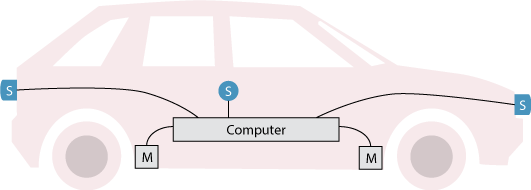
\includegraphics[width=12cm]{./media/overview.png}
	\caption{Konzept}
	\label{Fig1}
\end{figure}

Um sicherzugehen, welche Bauteile man braucht, und, wie sie alle zusammen funktionieren, haben wir im Internet unter [Quelle] nachgeschaut.
Wie wir uns dann entschieden haben, ist unter [Abschnitt Hardware] genauer dargestellt.

Wir haben die meiste Zeit zu dritt zusammen gearbeitet, f"ur die Dokumentation hat jeder einen Teilaspekt bearbeitet.
Die Aufteilung der Arbeit ist in Tabelle~\ref{Tab1} dargestellt.

\begin{table}[h]
	\centering
	\begin{tabular}{|l|l|}
	\hline
		Abschnitt & Person \\ \hline
		Abstract & Nicolas \\
		(1) Einf"uhrung & Nicolas \\
		(2.0) Haupteil & noch niemand \\
		(2.1) Hardware & Timo \\
		(2.2) Software & Quentin \\
		(3) Fazit und Ausblick & Nicolas \\
		alle Graphiken & Quentin \\
	\hline
	\end{tabular}
	\caption{Arbeitsteilung}
	\label{Tab1}
\end{table}

Im folgenden Hauptteil haben wir zuerst die Hardware, dann die Software behandelt.

\section{Hauptteil}\label{sec2}

die der Kollege Albert vom Patentamt Bern \cite{ModMyPi} auch schon beschrieben hat.

\begin{figure}[h]
	\centering
	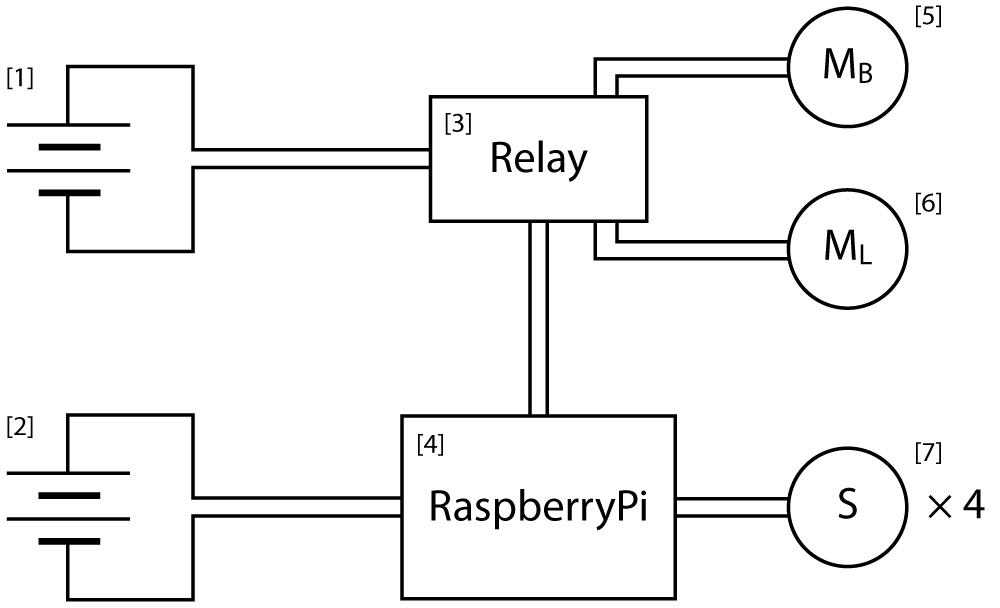
\includegraphics[width=10cm]{./media/circuit_general.png}
	\caption{grundlegender Schaltplan}
	\label{Fig2}
\end{figure}

\subsection{Hardware}\label{sec2.1}

In diesem Teil geht es um die Hardware des gesamten Projektes.
Die Hardware ist neben der Software der wichtigste Bestandteil des ganzen Projektes.
Ohne die Hardware w"are die Umsetzung nicht m"oglich gewesen, da wir kein Testobjekt h"atten, um Fehler herauszufinden.

Wir hatten uns also am Anfang, als wir uns ein Thema rausgesucht hatten, darum gek"ummert, was wir f"ur die Umsetzung br"auchten.
Also hatten wir uns an einem Abend auf Skype zusammengesetzt und dar"uber diskutiert.
Wir erkundigten uns auf Amazon "uber Produkte, welche wir eventuell kaufen w"urden.

\subsubsection{Finden der ben"otigten Teile}\label{sec2.1.1}

Wir "uberlegten uns, dass wir folgende Objekte brauchen w"urden, die essentiell waren, um passable Ergebnisse zeigen zu k"onnen:

\begin{myitemize}
	\item Modellauto mit Motor
	\item Computer, z.~B. Raspberry-Pi oder Arduino
	\item Akku f"ur Computer
	\item Kabel f"ur die Verbindungen
	\item Ultraschallsensoren f"ur Umgebungserfassung
\end{myitemize}

Wir haben uns dann f"ur ein Mini Cooper Modellauto in einen 1:30 Ma"sstab entschieden, f"ur einen Raspberry-Pi, f"ur einen 5600 mA/h Akku, Jumper-Stecker f"ur die Verbindungen und HC-SR04 Umgebungserfassungs-Module mit Ultraschall, welche extra f"ur den Raspberry-Pi abgestimmt waren.
Nach dieser Voreinsch"atzung, was wir f"ur Produkte brauchen, haben wir diese kurz danach bestellt.

Ungef"ahr einen Monat nachdem wir diese Komponenten bestellt hatten, kamen sie dann auch bei uns an. 

Aufbau/Beschreibung:
\begin{myitemize}
	\item Raspberry Pi:
	\begin{myitemize}
		\item 4 USB Ports
		\item 1 HDMI Port
		\item 1 Lan Port
		\item 1 Sound Port
		\item 1 Mikro USB Port  f"ur Akku
		\item 40 GPIO Pins zur Daten"ubertragung
	\end{myitemize}
	\item Akku:
	\begin{myitemize}
		\item Akkumulator
		\item USB- auf Mikro-USB-Kabel
	\end{myitemize}
	\item Breadboard:
	\begin{myitemize}
		\item Board f"ur Jumper-Stecker
	\end{myitemize}
	\item Jumper Stecker
	\item Ultraschallsensoren:
	\begin{myitemize}
		\item 4 Pins (GND, ECHO, VCC, TRIG)
		\item 1 Empf"anger
		\item 1 Sender
	\end{myitemize}
	\item Modellauto:
	\begin{myitemize}
		\item Chassis mit Motoren f"ur Steuern und Beschleunigen
		\item Karosserie aus Plastik nur Verzierung und Antenne
		\item Fernbedienung mit 4 Kn"opfen
	\end{myitemize}
\end{myitemize}

\subsubsection{Funktiontest der Komponenten}\label{sec2.1.2}

Wir hatten dann eine Funktions"uberpr"ufung durchgef"uhrt und gecheckt, ob die Komponenten auch funktionst"uchtig und einsatzbereit waren.
Dies haben wir getan indem wir in das Modellauto den geladenen Akku eingelegt hatten, die Fernbedienung startbereit gemacht hatten und das Auto angemacht hatten.
Beim ersten Anlauf hat es auf Anhieb sofort geklappt und wir konnten erste Messungen durchf"uhren, welche f"ur das sp"atere Vorgehen essentiell waren.
Wir haben das Auto auf die Stra"se gesetzt und haben es ca. 15- bis 20-mal fahren lassen.
Mithilfe von einer Stoppuhr und einer physikalischen Formel haben wir unterschiedliche Faktoren berechnet, dessen Ergebnisse wir selbstverst"andlich in unserem Laborbuch notiert haben:

\begin{myitemize}
	\item Geschwindigkeit: v = s/t:
	\begin{myitemize}
		\item $ \approx $ 2,34~m/s, raue Stra"se
		\item $ \approx $ 2,52~m/s, Fu"sweg/Steinplatten
	\end{myitemize}
	\item $ \frac{\pi}{2} $-Kurve:
	\begin{myitemize}
		\item $ \approx $ 0,29~rad $ \pm $ 0,02~rad Radneigung
		\item ca. 87 bis 90~cm (Stra"se), ca. 83 bis 85~cm (Fu"sweg) Hypotenuse f"ur $ \frac{\pi}{2} $-Kurve
	\end{myitemize}
	\item Bremsweg: $ < $ 5~cm
\end{myitemize}

Den Raspberry-Pi, den wir uns zugelegt hatten, hatten wir getestet, indem wir den vorher aufgeladenen Akku angeschlossen hatten, ein Betriebssystem mithilfe einer SD-Karte integriert hatten und mithilfe einiger simplen Befehle den Raspberry-Pi auf seine Funktion getestet hatten. 
Nachdem wir dann die Best"atigung hatten, dass der Raspberry-Pi funktionierte, war als n"achstes jeder der Ultraschallsensoren dran.
Dazu hatten wir sie einzeln an den Raspberry-Pi angeschlossen, indem wir jeden der Pins der Ultraschallsensoren zu einem dazu passenden Pin am Raspberry-Pi verbunden hatten.
Sprich der GND (Ground) Anschluss an den Ground Pin, den VCC (Stromversorgung) Anschluss an den Strom Pin und die ECHO und TRIG Anschl"usse wurden an jeweils an einen freien GPIO Pin angeschlossen.
Nun, da wir die Sensoren angeschlossen hatten, wurde sogleich die Reichweite und die Genauigkeit der einzelnen Sensoren getestet.
Aber wie genau diese Tests mit den einzelnen Codes ausgef"uhrt wurden, l"asst sich aus dem Abschnitt Software sehr gut herleiten.

Um all dies ordentlich ausf"uhren zu k"onnen, stand uns die gesamte Zeit ein Fernseher-Bildschirm und eine Tastatur zur Verf"ugung, um die Eingaben f"ur das Programm zu t"atigen und sie auf einer grafischen Oberfl"ache darstellen zu k"onnen.

Schnell stellten wir jedoch fest, als wir alle Ultraschallsensoren montieren wollten, dass der Rapberry-Pi nur zwei Stromversorgungspins hat.
Da wir aber vier Ultraschallsensoren hatten, ben"otigten wir entweder noch zwei Stromquellen oder eine andere L"osung.
Diese L"osung war dann, dass wir das Breadboard benutzt hatten um aus zwei Stromquellen vier zu machen.
Wir steckten die Jumper-Stecker in zwei verschiedenen Reihen in zwei Spalten und haben dann die vier Ultraschallsensoren jeweils in zwei aufgeteilt und auf die Stromanschl"usse verteilt.

Da wir uns nun im Klaren waren, dass alle Komponenten funktionierten, setzten wir uns daran, den Vorl"aufer des jetzigen Computerprogramms zu entwickeln.
Das Programm enthielt ausschlie"slich die Befehle f"ur die Ultraschallsensoren.

\subsubsection{Gestaltung des Fahrzeuginneren}\label{sec2.1.3}

Nachdem wir also die ersten Ans"atze des Programms geschrieben hatten, hatten wir uns Gedanken zur Unterbringung in dem, im Vergleich zur Technik, kleinen Modellauto gemacht.
Da das Auto zu einem Gro"steil aus Plastik besteht, war es eine Leichtigkeit das Auto zu bearbeiten.
Wir gingen also in die Werkstatt, die Erich Redweik (Timos Gro"svater) zur Verf"ugung stellte, in welcher wir die Werkzeuge vorfinden konnten, um solche Bearbeitungen durchzuf"uhren.
In der Werkstatt fanden wir eine Werkbank vor, sowie verschiedene Werkzeuge, unter anderem S"agen, Pfeilen, Schmirgelpapiere, H"ammer, Bohrer, Fr"asen, L"ot-Ger"ate und weitere Werkzeuge. Selbstverst"andlich waren dort auch Schutzbrillen vorzufinden.

Wir bearbeiteten das Auto nun so, dass alle unn"otigen Verzierungen im Auto wie Armaturenbrett und Sitze herauszunehmen waren.
Diese Teile schmissen wir dann weg, da wir sie nicht mehr brauchten.
Wir hatten Gl"uck mit dem Auto, da das Auto auf der nicht selbsttragenden Bauweise des Chassis basierte.
Das bedeutet, dass der obere Teil des Auto, sprich die Karosserie, nicht unbedingt n"otig war.
Deswegen konnten wir die Karosserie, in welcher auch Sitze und  Armaturenbrett eingebaut waren, einfach so bearbeiten, ohne Gefahr zu laufen wichtige Teile zu zerst"oren.
Wir trieben dann mit einem Schraubenzieher vier Schrauben durch das Dach des Modellautos und befestigten daran dann den Raspberry-Pi.
Im selben Arbeitsschritt integrierten wir dann auch noch das Breadboard und die Ultraschallsensoren, sowie die daf"ur wichtigen Jumper-Stecker.

\subsubsection{Relais}\label{sec2.1.4}

Nun war die Aufgabe, sich zu "uberlegen, wie wir die Signale der beiden Motoren, Steuerung und Antrieb, an den Raspberry-Pi weitergeben.
Wir testeten sehr viel aus, mit Jumper-Steckern, die die Signale weitergeben, mit der Platine, die im Auto vorhanden war, die wir versuchten mit dem Raspberry-Pi zu verbinden, aber all diese Versuche schlugen fehl und wir brauchten eine neue Idee.
Nach mehreren Stunden durchgehender "Uberlegungen, wie wir es anstellen k"onnten, und Recherchen im Internet, wurden wir immer noch nicht schlauer.
Irgendwann kam Timo auf die Idee, seinen Gro"svater Erich Redweik zu fragen, da jener als Industrie-Elektronik-Techniker gearbeitet hatte und wir uns erhofften, dass er uns helfen k"onnte.
Diese Idee wurde auch von Nicolas und Quentin positiv unterst"utzt und sofort wurde Herr Redweik angerufen und zu Rate gezogen.
Wir erkl"arten ihm das Problem welches wir hatten.

Das Problem war: Jeder der Motoren funktioniert so, dass die Spannung, welche auf den Motor gegeben wird, positiv oder negativ ist und damit die Richtung des Motors eingestellt wird, sprich, dass rechts-links Lenken oder vorw"arts-r"uckw"arts Fahren m"oglich ist.
Dass diese Motoren so funktionieren, wurde uns erst von Herr Redweik erkl"art.
Nun hatten wir das Problem, dass wir keine Ahnung hatten wie wir die Spannung mit Hilfe des Raspberry-Pi umkehren sollten.
Da erkl"arte uns Erich Redweik, dass das sehr einfach mit Hilfe eines Relais klappt.

Wir wussten nicht ganz, was so ein Relais ist, geschweige denn, wo wir so etwas herbekommen k"onnten.
Wir schauten es im Internet nach und fanden mit Hilfe von Wikipedia heraus, dass ein Relais ein fernbedienbarer Schalter sei, der durch elektrischen Strom betrieben wird und eine elektromagnetische Wirkung hat.
Im gleichen Arbeitsschritt schauten wir bei Online-H"andlern wie Amazon, Conrad, etc. nach, ob jene solche Relais besa"sen.
Da kein Laden in unserer N"ahe solche Relais besa"sen, rief Timo bei seinem anderen Opa in Essen an, Fritz Tillmann, da Timo wusste, dass dort eine Conrad-Filiale war.
Timo konnte erreichen, dass sein Opa ihm ein Relais besorgt und ihm per Post sendet.

Das Paket kam auch eine Woche sp"ater bei Timo zuhause an.
Die Relais, von denen wir vier St"uck auf einer Platine bekommen hatten, wurden direkt ausgepackt und in Betrieb genommen.
Wir verzichteten bei den Relais auf einen Test und bauten sie sofort ein.
Nach mehrmaligem Versuchen gelang es uns endlich, sie korrekt zu integrieren.

Die Relais wurden so angeschlossen, dass der VCC-Anschluss mit einem Jumper-Stecker zu den der Ultraschallsensoren hinzugef"ugt wurde, der GND-Anschluss mit einem Ground-Pin verbunden wurde und die Anschl"usse der einzelnen Relais-Schalter an jeweils einen GPIO-Pin.
Wir verbanden dann die beiden Motoren mit den Relais "uber das Breadboard und testeten dann, ob die Konstruktion funktionierte.

Da diese Tests einwandfrei funktionierten, wurde auch Platz f"ur die Relais-Platine gemacht und sie wurde mit Schrauben an dem Chassis montiert.
Als das geschafft war, wurde das Programm bearbeitet, sodass auch die Relais eingeschlossen waren.

\subsubsection{Erste Fahrversuche}\label{sec2.1.5}

Nun wurden die ersten richtigen Tests mit dem Auto durchgef"uhrt und getestet, ob die Motoren angesprochen werden konnten. Dann wurden auch die Ultraschallsensoren hinzugef"ugt.

Dann stieg die Spannung, weil wir die erste Fahrt mit dem Auto machten und das Auto auf eine Wand zufuhr und vor jener stehen bleiben sollte. Das Auto blieb im gew"unschten Abstand vor der Wand stehen und damit hatten wir unseren ersten Erfolg erzielt.

\subsubsection{Kurven}\label{sec2.1.6}

\subsection{Software}\label{sec2.2}

F"ur die Steuerung des Autos haben wir ein Programm geschrieben, welches auf dem von uns im Auto eingebauten Raspberry Pi ausgef"uhrt wird.
Bei der Auswahl der Programmiersprache konnten wir uns, auf Grund unseres Vorwissens und der technischen Limitierung des Raspberry Pi, lediglich zwischen Python und C++ entscheiden.
Wir haben uns dann f"ur Python entschieden; vorallem auf Grund der einfachen Syntax, welche uns schnellere "Anderungen am Programm-Code erlaubt.

Die grundlegende Aufgabe des Programms ist es, zuerst Messungen mittels der Ultraschallsensoren durchzuf"uhren, diese Messungen auszuwerten, und dann entsprechende Signale an die Motoren des Autos zu senden.

\medskip

Im folgenden beschreibe ich den grundlegenden Aufbau des Programms.
Zuerst definieren wir ein paar Konstanten, die in dem Programm h"aufiger verwendet werden, etwa den Umrechnungsfaktor, mit dem wir aus der Zeit, die das Ultraschallsignal braucht, die Enfernung des Objektes berechnen k"onnen und umgekehrt.
Diesen Wert haben wir zuerst durch einen einfachen Versuch herausfinden m"ussen.
Wir haben Objekte in bestimmten Entfernungen des Autos gestellt, und Messungen durchgef"uhrt.
Dies haben wir f"ur Objekte in verschiedenen Entfernungen durchgef"uhrt, sodass wir schlie"slich durch den Quotienten aus Strecke und Zeit den Umrechnungsfaktor errechnen konnten.
Oder auch die von uns festgelegte maximale Abweichung, die ein Wert haben darf, ohne als Fehlerwert zu gelten.
Und auch die Nummern der von uns verwendeten Pins am Raspberry Pi speichern wir in Konstanten, damit wir diese nachher einfacher abrufen k"onnen und die jeweilige Zahl nur ein einziges mal im Code vorkommt.
Somit muss bei einem Umstecken der Verbindungen nur eine Zahl ge"andert werden.

Au"serdem deklarieren wir einige Variablen, die wir verwenden k"onnen, um w"ahrend der Ausf"uhrung des Programms Werte zwischenzuspeichern.
Die wichtigsten dieser Variablen sind unsere vier Listen.
In der Liste RESULT speichern wir die letzten Werte, die die Ultraschallsensoren gemessen haben, das hei"st die Zeiten zwischen Senden des Ultraschallsignals und erneuten Empfangen desselben, und den dazugeh"origen Zeitpunkt, zu dem die Messung stattgefunden hat.
In dieser Liste sind immer nur die letzten Messwerte gespeichert, bis sie auf Fehler "uberpr"uft wurden.
Wenn sie nach der "Uberpr"ufung als Fehlerwert gelten, d.~h. eine zu gro"se Abweichung von dem vorigen Messwert haben, kommen sie in die Liste WDATA.
In dieser werden die Werte dann erneut f"ur eine weitere "Uberpr"ufung zwischengespeichert, bei dieser werden die letzten Messwerte je mit den Werten aus der vierten Liste verglichen.
Das hei"st es wird letztendlich "uberpr"uft, ob sich die letzten Messwerte, nachdem ein Fehler erkannt wurde, stark genug "ahneln um doch als richtige Werte zu gelten.
Sobald die Werte nach einer "Uberpr"ufungen als richtige Werte angesehen werden, werden die Messwerte in die Liste DATA "uberf"uhrt und die dazugeh"origen Zeitpunkte in die Liste TIME.
Die Werte aus diesen beiden Listen k"onnen letztendlich in Entfernungen umgerechnet werden und so weiterverwendet werden, etwa f"ur die Berechnung der Geschwindigkeit oder f"ur das Einleiten eines Bremsvorganges, wenn das Hindernis dem Auto zu nahe kommt.
Auf Grund von Fehlerwerten, die nicht als Messwerte aufgennommen werden, sind die Messungen nicht zwangsl"aufig in gleichm"a"sigen Zeitabst"anden.
In diesen F"allen wird der Zeitpunkt der Messung ben"otigt um bestimmte Berechnungen, wie etwa die Errechnung der Geschwindigkeit, durchzuf"uhren.

\medskip

Beim Ausf"uhren des Programms wird zuerst unsere Hauptmethode aufgerufen, innerhalb dieser werden dann der Reihe nach einige spezialisierte Funktionen aufgerufen, welche sich jeweils mit einem Arbeitsschritt befassen.
Etwa die Methode measure(i), welche eine Messung mit dem Sensor i durchf"uhrt und das Ergebnis abspeichert.
Wobei i die Nummer des Sensors ist (wir haben diese von 0 bis 3 durchnummeriert).
Diese Funktionen werde ich im Folgenden einzeln erl"autern.

\subsubsection{setup()}\label{sec2.2.1}
\lstinputlisting[language=Python, firstline=30, lastline=46]{../main.py}
Diese Funktion wird als erstes ausgef"uhrt, wenn das Hauptprogramm gestartet wird.
Sie ist daf"ur zust"andig, alle Pins wieder auf ihren Ausgangszustand zur"uckzusetzen, d.~h. die Pins auf OUT bzw. IN zu stellen und die angelegte Spannung der OUT-Pins auf 0~V zu setzen.
Au"serdem werden die Einstellungen der GPIO Library gesetzt.
Die GPIO Library haben wir als Schnittstelle zwischen unserem Programm und den Pins des Raspberry Pi gew"ahlt.
Durch Funktionsaufrufe an diese Library k"onnen wir ablesen, ob an den IN-Pins eine Spannung von 3,5~V anliegt, und wir k"onnen an den OUT-Pins selbst eine Spannung von 3,5~V anlegen.

\subsubsection{driveForward()}\label{sec2.2.2}
\lstinputlisting[language=Python, firstline=143, lastline=149]{../main.py}
Beim Aufruf dieser Funktion f"angt das Auto an zu fahren.
Dies wird durch eine "Anderung der Spannungen an den Pins, die "uber das Relais am Antriebsmotor angeschlossen sind, erreicht.
Diese "Anderung sorgt letztendlich daf"ur, dass ein geschlossener Stromkreis zwischen dem Akku des Autos und dem Antriebsmotor entsteht, und, dass eine positive Spannung an diesem anliegt.
Das daf"ur sorgt, dass das Auto beginnt vorw"arts zu beschleunigen.
Dementsprechend gibt es auch noch die Funktionen driveBackward(), stopdrive(), steerLeft(), steerRight() und stopsteer(), die im Grunde alle auf die gleiche Art und Weise funktionieren.
Diese Funktionen sind, entsprechend ihrer englischen Namen, f"ur das R"uckw"artsfahren, Stoppen und Lenken verantwortlich.

\subsubsection{brake()}\label{sec2.2.3}
\lstinputlisting[language=Python, firstline=180, lastline=192]{../main.py}
F"ur das Bremsen allerdings hat uns ein einfaches Aufrufen von stopdrive() nicht gereicht.
Dabei wird der Antriebsmotor lediglich ausgeschaltet, was einen relativ langsamen Bremsvorgang zur Folge hat.
Eine bessere Methode ist diese Funktion.
Im Gegensatz zu einem einfachen Ausschalten des Motors wirkt diese Funktion der aktuellen Bewegungsrichtung f"ur einen kurzen Moment, mithilfe des Antriebsmotors, entgegen.
Dies sorgt f"ur einen deutlich schnelleren Bremsvorgang.

\subsubsection{measure(i)}\label{sec2.2.4}
\lstinputlisting[language=Python, firstline=54, lastline=81]{../main.py}
Der Parameter i in dieser Funktion beschreibt den Sensor, mit dem gemessen werden soll.
Dabei handelt es sich bei i um eine Zahl von 0 bis 3.
Zuerst f"uhrt diese Funktion eine Messung mit dem angegebenen Sensor durch.
Danach wird der erhaltene Messwert in der Liste RESULT abgespeichert.
Um eine Messung mit dem Ultraschallsensor zu starten, muss man diesem zuerst "uber den daran angeschlossenen OUT-Pin einen elektrischen Impuls der Dauer 10~µs und Spannung 3,5~V geben.
Dann wartet unser Programm auf eine R"uckmeldung von dem Sensor, dies Erfolgt durch einen "ahnlichen elektrischen Impuls, den wir "uber den IN-Pin, der mit dem Sensor verbunden ist, empfangen k"onnen.
Den Zeitpunkt, zu dem wir diesen Impuls empfangen haben, speichern wir zwischen, da dieser genau dem Zeitpunkt entspricht, zu dem das Ultraschallsignal gesendet wurde.
Entsprechend dem ersten kommt dann, bei Empfangen des Ultraschallsignals, ein weiterer Impuls, den wir erneut empfangen und dessen Zeitpunkt abspeichern, sodass wir schlie"slich durch die Differenz der beiden Zeitpunkte die Zeit herausfinden, die das Ultraschallsignal f"ur Hin- und R"uckweg gebraucht hat.
Hierbei haben wir au"serdem einen Schutz eingebaut, der das Programm davor sch"utzt, in einer Messung unendlich lang auf den zweiten Impuls zu warten.
Und zwar wird das Warten auf den zweiten Impuls nach 25~ms abgebrochen.
Falls dies passiert, wird als gemessener Zeitwert -1 abgespeichert, dies behandeln wir im Programm allgemein als fehlgeschlagene Messungen.

\subsubsection{check\_results(i)}\label{sec2.2.5}
\lstinputlisting[language=Python, firstline=108, lastline=136]{../main.py}
Bereits bei den ersten Tests ist uns aufgefallen, dass relativ h"aufig fehlerhafte Werte auftreten.
Deshalb war uns schon ziemlich fr"uh klar, dass wir eine Funktion brauchen, die die Messwerte auf ihre Richtigkeit "uberpr"uft.
W"urden diese Werte etwa in der Abstands"uberpr"ufung verwendet, so k"onnte dies dazu f"uhren, dass das Auto zu fr"uh bremst.
Zuerst "uberpr"uft die Funktion, ob die Differenz zwischen dem zuletzt gemessenen Wert und dem zuletzt als g"ultigen Wert Abgespeichertem nicht unsere Maximalabweichung "uberschreitet.
Diese Maximalabweichung haben wir als Konstante mit dem Wert 0,2~m definiert.
Ist diese Abweichung geringer als das von uns festgelegte Maximum, so wird der zuletzt gemessene Wert ohne weitere "Uberpr"ufungen als g"ultiger Wert angesehen und abgespeichert.
Andernfalls gibt es zwei verschiedene M"oglichkeiten.
Entweder ist war der vorige Wert g"ultig, dann wird der zuletzt gemessene Wert ohne weiteres in der Liste WDATA abgelegt.
Oder aber einer oder mehrere vorangegangene Werte waren bereits ebenfalls ung"ultig, dann wird der zuletzt gemessen Wert erst noch mit diesen Werten verglichen.
Wenn dann die drei letzten Werte nah beieinander lagen, d.~h. die Differenz nicht die Maximalabweichung "uberschreitet, dann wird der zuletzt gemessene Werte als g"ultiger Messwert angesehen, und dementsprechend in der Liste DATA abgespeichert.
Anschlie"send wird aus den letzten zwei g"ultigen Messungen die momentane Geschwindigkeit berechnet.
Au"serdem schreibt die Funktion f"ur jede fehlgeschlagene Messung (Wert -1) und jeden abweichenden Messwert einen Kommentar in die Logfile.

\subsubsection{turn(a)}\label{sec2.2.6}
\lstinputlisting[language=Python, firstline=195, lastline=206]{../main.py}
Mit Hilfe dieser Funktion wollten wir es m"oglich machen Kurven mit einem festen Winkel zu fahren, dabei w"urde dann der Parameter a den Winkel in Grad angeben.
Allerdings hat dies nicht ganz funktioniert, auch wenn wir ohne Probleme mit Hilfe von steerLeft() und steerRight() einlenken konnten, hat es doch nicht funktioniert Kurven des angegebenen Winkels zu fahren.
Stattdessen ist das Auto die Kurven zu weit oder nicht weit genug gefahren.
Weshalb diese Funktion in unserem Hauptprogramm drive1() auch nicht verwendet wird, sondern nur in unserer Testmethode drive2().
Da wir beim Motor, der f"ur die Lenkung zust"andig ist, lediglich nach links oder rechts lenken k"onnen (immer der gleiche Einschlagwinkel), konnten wir die Weite der Kurve nur durch die Dauer des Einlenkens beeinflussen.
Dabei ist es vermutlich zu Probleme gekommen, weil wir f"ur die Berechnung dieser Dauer die Geschwindigkeit verwendet haben, die das Auto hatte als es anf"angt die Kurve zu fahren.
Wenn sich dann allerdings die Geschwindigkeit w"ahrend dem Fahren der Kurve "ander, dann beeinflusst dies die Weite der Kurve.
Stattdessen h"atten wir f"ur eine genauere Methode, entweder durchgehend die Geschwindigkeit des Autos bestimmen m"ussen, oder wir h"atten eine andere Methode finden m"ussen, um zu bestimmen wann das Auto die Kurve zu Ende gefahren hat.

\subsubsection{countdown(t)}\label{sec2.2.7}
\lstinputlisting[language=Python, firstline=209, lastline=214]{../main.py}
Diese Funktion existiert lediglich aus praktischen Gr"unden.
Und zwar ist es uns momentan nur m"oglich das Programm "uber eine angeschlossene Tastatur zu starten.
Da das Auto sofort nach starten des Programms zu fahren beginnt, und das Kabel der angeschlossenen Tastatur f"ur die Fahrtests eine deutliche Einschr"ankung darstellt, ist diese Funktion daf"ur zust"andig eine, durch t bestimmte, Zeit in Sekunden zu warten.
Diese Funktion starten wir also, vor dem Start von drive1(), um ein wenig Zeit zu haben bevor das Auto losf"ahrt.

\subsubsection{Gesamter Quelltext}\label{sec2.2.8}
\lstinputlisting[language=Python, firstline=1, lastline=272]{../main.py}

\section{Fazit und Ausblick}\label{sec3}

Wir haben es geschafft, dass das Auto geradeaus fahren kann.
Das ist ein Teilerfolg, aber das urspr"ungliche Ziel (einen Parkours zu fahren) haben wir nicht erreicht.

Besondere Probleme haben uns die Kurven bereitet. ...

Au"serdem hatten wir Schwierigkeiten, bei dem immer komplexer werdenden Programm den "Uberblick zu behalten.
Wir haben den Aufwand und die Komplexit"at des Programms zuerst untersch"atzt.
Wir haben mehrmals versucht, einen hinreichenden Logfile zu implementieren; letztendlich hat es aber nicht gereicht, um die aufgetretenen Fehler zu identifizieren.

Wir haben nicht verstanden, wof"ur die uns empfohlenen [siehe ...] Widerst"ande gut sein sollen.
Vielleicht hat dieser Umstand auch einige Probleme verursacht, zum Beispiel bei den Messungen von den Ultraschallsensoren?

Die hardwareseitige Entwicklung lief weitgehend zufriedenstellen.
Wir haben schnell den Aufbau und die Funktionsweise des Autos verstanden und konnten alle unsere "Uberlegungen umsetzen.

Wenn wir mehr Zeit h"atten, w"urden wir das Programm komplett neu schreiben und besonders auf ausreichende Logfile-Ausgaben achten.
Danach k"onnte man nocheinmal versuchen, das Auto Kurven fahren zu lassen.

\bigskip


\addcontentsline{toc}{section}{Literatur}
\begin{thebibliography}{99}
	\itemsep-2pt \small
	\bibitem{ModMyPi} http://www.modmypi.com/blog/hc-sr04-ultrasonic-range-sensor-on-the-raspberry-pi
\end{thebibliography}

\newpage


{\large\bf Danksagung}

\medskip

blabla

\bigskip


{\large\bf Erkl"arung der Eigenst"andigkeit}

\medskip

blabla

\end{document}
